\subsection{Effectiveness of Training Data Synthesis}
\label{subsec:data_effectiveness}

\begin{figure}[t]
    \centering
    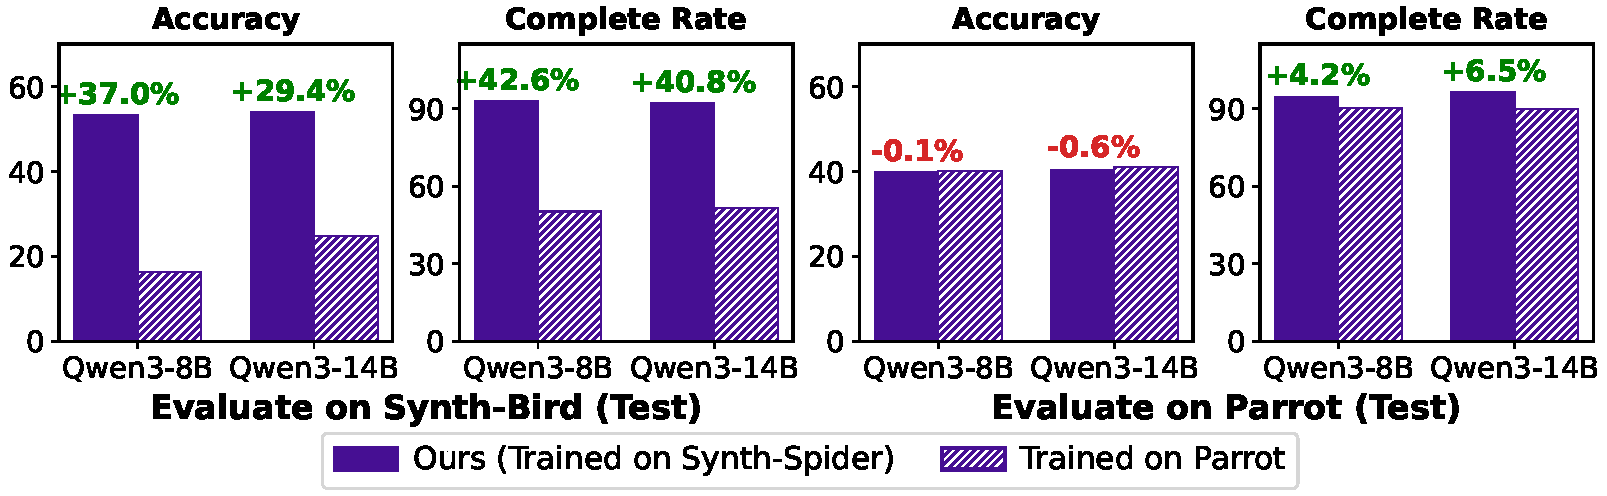
\includegraphics[width=1.01\columnwidth]{plots/plot/trained_on_spider_and_parrot.pdf}
    \vspace{-2em} 
    \caption{Evaluation results of models trained on Synth-Spider (Train) and Parrot (Train).}
    \label{\labelprefix fig:trained_on_spider_and_parrot}
    \vspace{-1em}
\end{figure}
\begin{figure}[t]
    \centering
    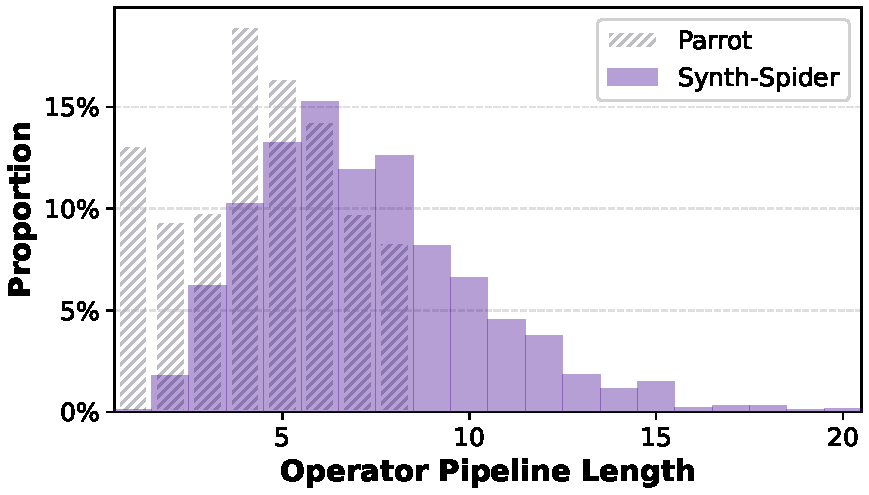
\includegraphics[width=0.95\columnwidth]{plots/plot/op_len_distribution.pdf}
    \vspace{-1em} 
    \caption{Operator Pipeline Length Distribution.}
    \label{fig:op_len_distribution}
    \vspace{-0.5em}
    % \vspace{-1em}
\end{figure}


\stitle{Exp-\expnum\label{exp:data_effectiveness}: Effectiveness of Synthesized Training Data.}
We evaluate whether models trained on our synthesized Synth-Spider training set generalize comparably to those trained on the public Parrot training set. Both models are evaluated on the Parrot test set.

Figure~\ref{fig:trained_on_spider_and_parrot} shows that training on Synth-Spider achieves accuracy close to training on Parrot, with only small differences (0.10 and 0.60 for Qwen3-8B and Qwen3-14B, respectively). At the same time, completion rate is higher when training on Synth-Spider, with gains of 4.20 and 6.50 points across the two model sizes. These results indicate that the synthesized training tasks are effective for learning ADP pipelines and transfer well to a public benchmark.
To better understand this difference, we compare the operator pipeline length distributions of the two training datasets (Figure~\ref{fig:op_len_distribution}). Parrot training samples are concentrated on shorter pipelines, while Synth-Spider includes more medium- and long-horizon pipelines. This aligns with the observed completion rate gains, as models trained on longer pipelines show more stable multi-step execution and fewer early termination failures on the Parrot test set.

%Figure~\ref{fig:trained_on_spider_and_parrot} illustrates the evaluation results on the test set of Parrot. 
%We observe that models trained on Synth-Spider maintain comparable accuracy to the in-domain baseline. 
%The performance gap is trivial. 
%Specifically, Qwen3-8B and Qwen3-14B show marginal accuracy decreases of only 0.10 and 0.60 respectively. 
%In contrast, the Completion Rate exhibits a significant improvement. 
%Our approach achieves gains of 4.20 and 6.50 across the two model sizes. 
%
%To explain this phenomenon, we analyze the distribution of operator pipeline lengths in %both datasets, as shown in Figure~\ref{fig:op_len_distribution}.
%The public Parrot dataset exhibits a distribution concentrated on tasks with shorter operator pipelines
%When training samples are predominantly short, the model tends to overfit to shallow heuristics rather than learning to plan and recover from errors. 
%Conversely, our dataset contains a substantial proportion of samples requiring between 10 and 20 operators. 
%This forces the model to develop robust multi-step planning and global error correction mechanisms. 
%Consequently, even when evaluated on unseen tasks in Parrot, the model trained on Synth-Spider generates plans that strictly align with target schema. 
%Furthermore, when encountering execution errors, it generate comprehensive recovery strategies.

\begin{shaded}
\noindent \textbf{Finding \findingnum: 
Our synthetic training data provides effective supervision for agentic training, improving completion rate on unseen tasks while maintaining comparable accuracy.
%Our data synthesis strategy fosters robust planning, significantly improving task completion rates on unseen tasks without compromising accuracy.
}
\end{shaded}